\section{Experiments}
\label{sec:experiments}
\begin{figure*}
	\centering
	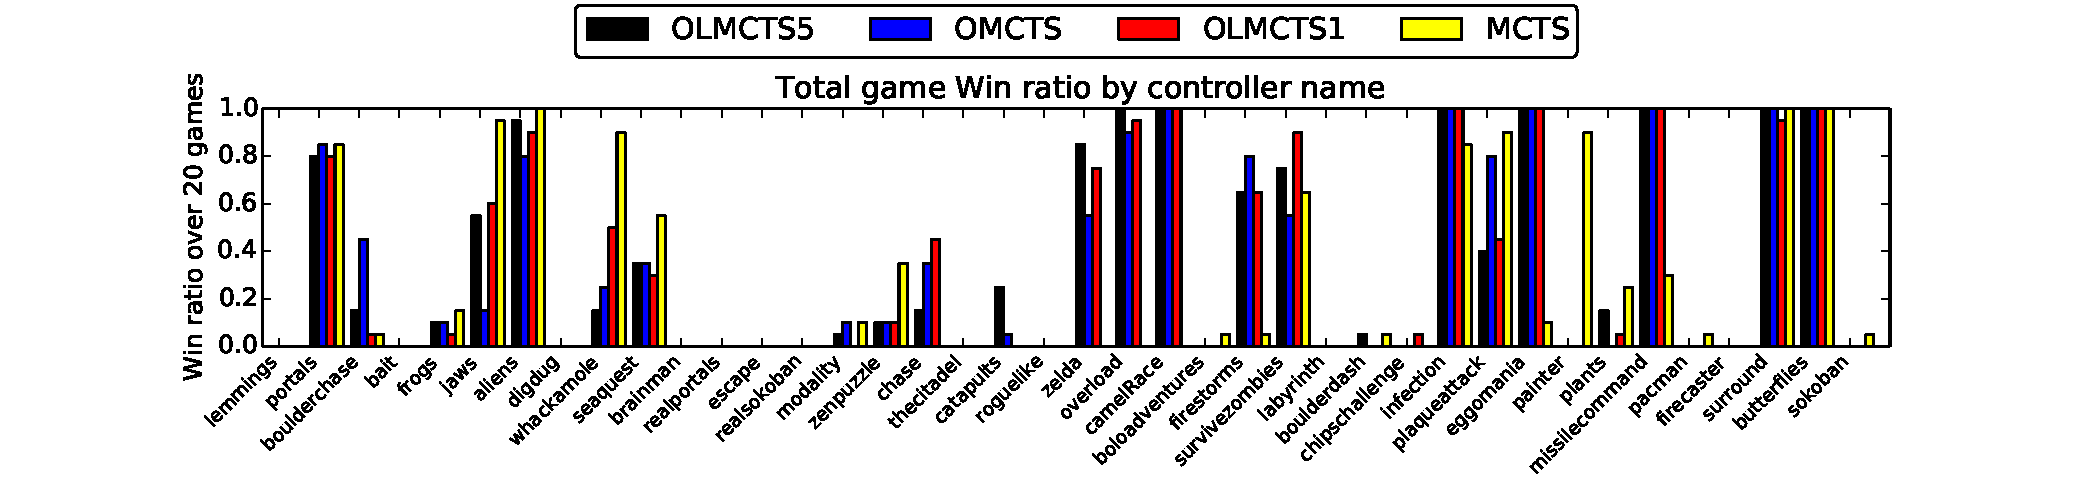
\includegraphics[width=\textwidth]{includes/wins}
	\vspace{-.8cm}
	\caption{Win ratio of the algorithms per game on all levels.}
	\label{fig:wins}
\end{figure*}

\begin{figure*}
	\centering
	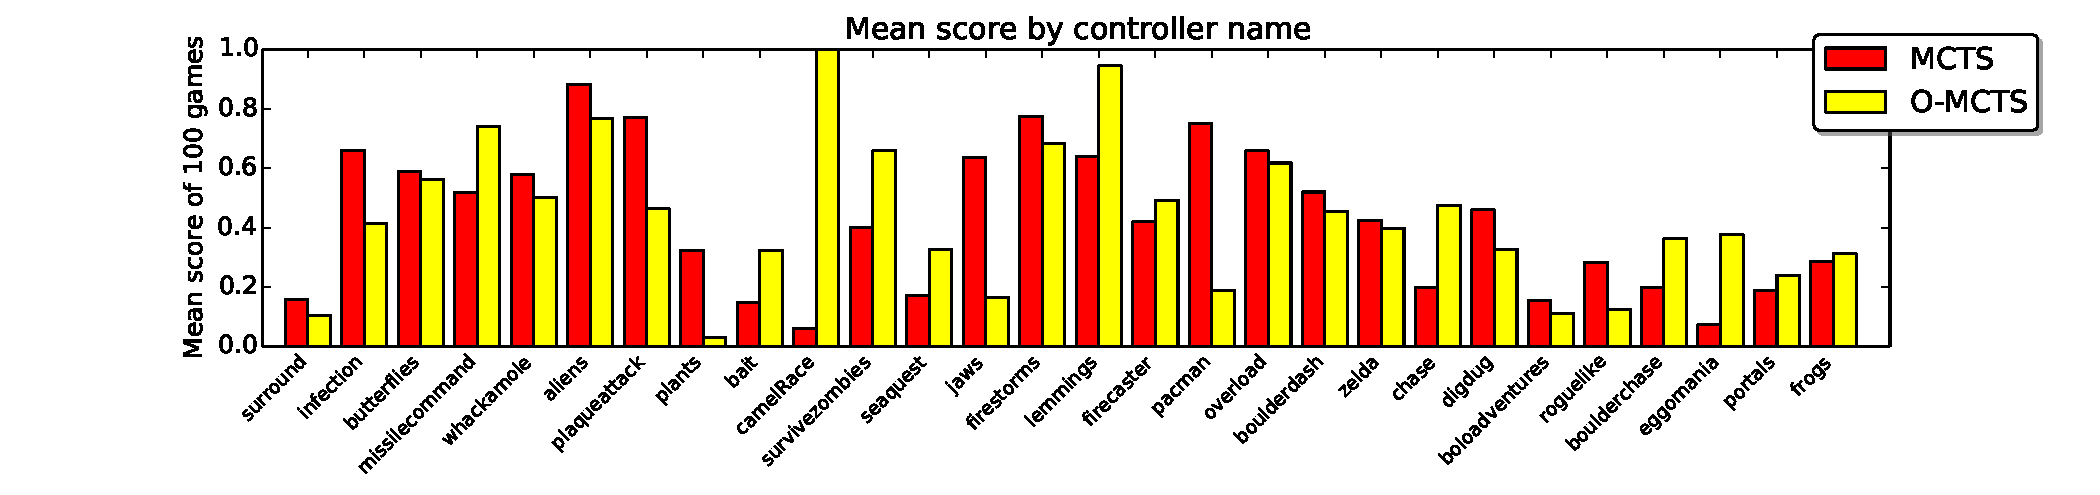
\includegraphics[width=\textwidth]{includes/scores}
	\vspace{-.8cm}
	\caption{Mean normalized score of the algorithms per game 1 means the
	highest score achieved by all the algoriths, 0 the lowest.}
	\label{fig:scores}
\end{figure*}


In this section we compare O-MCTS and OL-MCTS to traditional MCTS by running
simulations on 28 different games in the VGDL framework. These games include all
games from the first four training sets of the GVGAI competition, excluding the
puzzle games that can be solved by a simple exhaustive search. For this
experiment we constructed the following option types. More options can be
created and added to the algorithm easily.

\begin{itemize}[noitemsep]
	\item \texttt{ActionOption} executes a specific action once and then
		stops.
	\item \texttt{AvoidNearestNpcOption} makes the agent avoid the nearest NPC
	\item \texttt{GoNearMovableOption} makes the agent walk towards a
		movable game sprite (defined as movable by the VGDL) and stops when it
		is within a certain range of the movable
	\item \texttt{GoToMovableOption} makes the agent walk towards a
		movable until its location is the same as that of the movable
	\item \texttt{GoToNearestSpriteOfType} makes the agent walk to the nearest sprite of
		a specific type
	\item \texttt{GoToPositionOption} makes the agent walk to a specific position
	\item \texttt{WaitAndShootOption} waits until an NPC is in a specific location and
		then uses its weapon.
\end{itemize}

For each option type, a subtype per sprite type is created during the game. For
each sprite, an option instance of its corresponding subtype is created. For
example, the game Zelda, as seen in Figure \ref{fig:zelda}, contains three
different sprite types (excluding the avatar and walls); monsters, a key and a
portal. The first level contains three monsters, one key and one portal, and the
aim of the game is to collect the key and walk towards the portal without
walking into the monsters. \texttt{GoToMovableOption} and
\texttt{GoNearMovableOptions} will be created for each of the three monsters and
for the key. A \texttt{GoToPositionOption} will be created for the portal.  One
\texttt{GoToNearestSpriteOfType} will be created per sprite type. One
\texttt{WaitAndShootOption} will be created for the monsters, and one
\texttt{AvoidNearestNpcOption} will be created. This set of options is $O$ in
Algorithms \ref{alg:omcts} and \ref{alg:olmcts}.

The \texttt{GoTo\ldots} options all utilize an adaptation of the A Star
algorithm to plan routes. An adaptation was needed, because at the
beginning of the game there is no knowledge of which sprites are traversable and
which are not. Thus, during every move that is simulated by the agent, the A
Star module has to update its beliefs about the location of walls and other
blocking objects. It does so by comparing the movement the avatar wanted to make
to the movement that was actually made in game. If the avatar did not move and
did not change direction, it is assumed that all the sprites on the location the
avatar should have ended up in are blocking sprites. A Star keeps a \emph{wall
score} for each sprite type. When a sprite blocks the avatar, its wall score is
increased by one. Additionally, when a sprite kills the avatar, its wall score
is increased by 100, in order to prevent the avatar from walking into killing
sprites. Traditionally, for the A Star's heuristic, the distance between two
points is calculated. This version of A Star adds the wall score of the location
being investigated to this heuristic, encouraging the algorithm to take paths
with a lower wall score. This method enables A Star to try to traverse paths
that were unavailable earlier. For example, if a door is closed until a key is
picked up, this A Star algorithm will still be able to plan a path to the door,
once the key is picked up, winning the game.

The O(L)-MCTS algorithm has some parameters, which were empirically optimized
for these experiments. We use discount factor $\gamma = 0.9$, maximum action
time $t = 40$ milliseconds. The maximum search depth $d$ is set to 80, which is
higher than most alternative tree search algorithms, e.g.  the competitors in
the GVGAI competition, use. The number of node visits after which \textsf{uct} is
used, $v$, is set to 40. Crazy stone parameter $K$ is set to $0.5$.
For comparison, we use the MCTS algorithm provided with the Java implementation
of VGDL with its default value of maximum search depth of 8. Both algorithms
have \textsf{uct} constant $C_p = \sqrt{2}$.

We ran the algorithms on a set of 40 different games with 5 levels each. For
each level, we use the mean results of 20 plays. For the transfer learning
algorithm the fifth game after 4 training games was used (it played 100
games per level altogether).

Figures \ref{fig:wins} and \ref{fig:scores} respectively show the win ratio and
normalized score for each game and algorithm. As can be seen in Figure
\ref{fig:wins}, the O-MCTS algorithms performs at least as good as MCTS in
almost all games. 

Big wins for the MCTS algorithm can be seen in whackamole, jaws and plaque
attack. The similarity of these games is that they have a very big number of
different sprites, for each of which several options have to be created.
When the number of options becomes too big, constructing the initiation set of
options $\mathbf{p}_s$ for every state $s$ becomes so time-consuming that the
algorithm has too little time to build a tree and find the best possible
action.

Contrarily, O-MCTS greatly outperforms MCTS in the games missile command,
overload, firestorms, zelda, camel race, eggomania, firecaster and chase. If we
inspect the algorithm's performance for these games, we can see that the
algorithm succeeds in efficiently planning paths in a dangerous environment,
enabling it to do a further forward search than the ordinary Monte Carlo tree
search. Camel race requires the player to move to the right for 80 consecutive
turns, which is very hard for MCTS, since it only looks forward 8 turns. O-MCTS
almost always wins, since it can plan forward a lot further. In Overload, a
sword has to be picked up before the avatar can finish the game, which seems to
be too hard for MCTS, but poses less of a problem for O-MCTS.

\begin{figure}
	\centering
	\subfigure[Learning \textit{bait}]{
		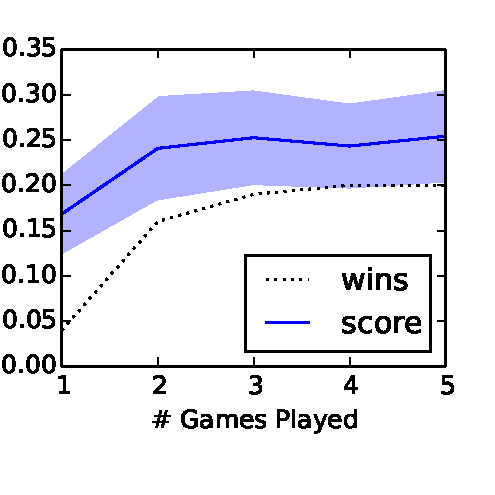
\includegraphics[scale=.44]{includes/learning}
		\label{fig:learning-results}
	}
	\subfigure[Totals]{
		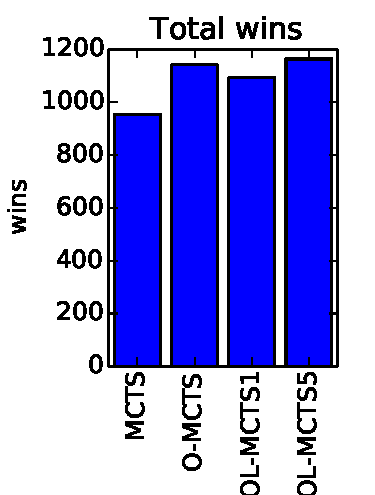
\includegraphics[scale=.44]{includes/totals.pdf}
		\label{fig:total-results}
	}
	\caption{Learning improvement and total number of wins of the algorithms on
	all games.}
\end{figure}

Furthermore, the graph shows that the transfer learning algorithm
significantly improves score over the course of 5 plays of bait. Bait is a game
in which the objective is to reach a goal portal after collecting a key. The
player can push boxes around to open paths. There are holes in the ground that
kill the player, unless they are filled with boxes, which make both the hole and
the box disappear. The improvement in score (including variance) and wins for
this game are shown in Figure \ref{fig:learning-results}. There are three
possible reasons for this improvement: 1.) There are sprites that kill the
player, which will be evaded by the algorithm when it has learned to do so.
2.) The algorithm might learn that it should pick up the key. 3.) The
player might learn to apply options in such a way that he can push boxes into the
(deadly) holes.

Figure \ref{fig:total-results} shows the sum of wins over all games, all levels.
It shows a significant ($p < 0.05$) improvement of O-MCTS, OL-MCTS and OTL-MCTS
over MCTS. Unfortunately, no significant difference can be found for all games
by incorporating learning.
